% Options for packages loaded elsewhere
\PassOptionsToPackage{unicode}{hyperref}
\PassOptionsToPackage{hyphens}{url}
%
\documentclass[
]{article}
\usepackage{amsmath,amssymb}
\usepackage{lmodern}
\usepackage{ifxetex,ifluatex}
\ifnum 0\ifxetex 1\fi\ifluatex 1\fi=0 % if pdftex
  \usepackage[T1]{fontenc}
  \usepackage[utf8]{inputenc}
  \usepackage{textcomp} % provide euro and other symbols
\else % if luatex or xetex
  \usepackage{unicode-math}
  \defaultfontfeatures{Scale=MatchLowercase}
  \defaultfontfeatures[\rmfamily]{Ligatures=TeX,Scale=1}
\fi
% Use upquote if available, for straight quotes in verbatim environments
\IfFileExists{upquote.sty}{\usepackage{upquote}}{}
\IfFileExists{microtype.sty}{% use microtype if available
  \usepackage[]{microtype}
  \UseMicrotypeSet[protrusion]{basicmath} % disable protrusion for tt fonts
}{}
\makeatletter
\@ifundefined{KOMAClassName}{% if non-KOMA class
  \IfFileExists{parskip.sty}{%
    \usepackage{parskip}
  }{% else
    \setlength{\parindent}{0pt}
    \setlength{\parskip}{6pt plus 2pt minus 1pt}}
}{% if KOMA class
  \KOMAoptions{parskip=half}}
\makeatother
\usepackage{xcolor}
\IfFileExists{xurl.sty}{\usepackage{xurl}}{} % add URL line breaks if available
\IfFileExists{bookmark.sty}{\usepackage{bookmark}}{\usepackage{hyperref}}
\hypersetup{
  pdftitle={DAP Project},
  pdfauthor={Daniel Granja},
  hidelinks,
  pdfcreator={LaTeX via pandoc}}
\urlstyle{same} % disable monospaced font for URLs
\usepackage[margin=1in]{geometry}
\usepackage{color}
\usepackage{fancyvrb}
\newcommand{\VerbBar}{|}
\newcommand{\VERB}{\Verb[commandchars=\\\{\}]}
\DefineVerbatimEnvironment{Highlighting}{Verbatim}{commandchars=\\\{\}}
% Add ',fontsize=\small' for more characters per line
\usepackage{framed}
\definecolor{shadecolor}{RGB}{248,248,248}
\newenvironment{Shaded}{\begin{snugshade}}{\end{snugshade}}
\newcommand{\AlertTok}[1]{\textcolor[rgb]{0.94,0.16,0.16}{#1}}
\newcommand{\AnnotationTok}[1]{\textcolor[rgb]{0.56,0.35,0.01}{\textbf{\textit{#1}}}}
\newcommand{\AttributeTok}[1]{\textcolor[rgb]{0.77,0.63,0.00}{#1}}
\newcommand{\BaseNTok}[1]{\textcolor[rgb]{0.00,0.00,0.81}{#1}}
\newcommand{\BuiltInTok}[1]{#1}
\newcommand{\CharTok}[1]{\textcolor[rgb]{0.31,0.60,0.02}{#1}}
\newcommand{\CommentTok}[1]{\textcolor[rgb]{0.56,0.35,0.01}{\textit{#1}}}
\newcommand{\CommentVarTok}[1]{\textcolor[rgb]{0.56,0.35,0.01}{\textbf{\textit{#1}}}}
\newcommand{\ConstantTok}[1]{\textcolor[rgb]{0.00,0.00,0.00}{#1}}
\newcommand{\ControlFlowTok}[1]{\textcolor[rgb]{0.13,0.29,0.53}{\textbf{#1}}}
\newcommand{\DataTypeTok}[1]{\textcolor[rgb]{0.13,0.29,0.53}{#1}}
\newcommand{\DecValTok}[1]{\textcolor[rgb]{0.00,0.00,0.81}{#1}}
\newcommand{\DocumentationTok}[1]{\textcolor[rgb]{0.56,0.35,0.01}{\textbf{\textit{#1}}}}
\newcommand{\ErrorTok}[1]{\textcolor[rgb]{0.64,0.00,0.00}{\textbf{#1}}}
\newcommand{\ExtensionTok}[1]{#1}
\newcommand{\FloatTok}[1]{\textcolor[rgb]{0.00,0.00,0.81}{#1}}
\newcommand{\FunctionTok}[1]{\textcolor[rgb]{0.00,0.00,0.00}{#1}}
\newcommand{\ImportTok}[1]{#1}
\newcommand{\InformationTok}[1]{\textcolor[rgb]{0.56,0.35,0.01}{\textbf{\textit{#1}}}}
\newcommand{\KeywordTok}[1]{\textcolor[rgb]{0.13,0.29,0.53}{\textbf{#1}}}
\newcommand{\NormalTok}[1]{#1}
\newcommand{\OperatorTok}[1]{\textcolor[rgb]{0.81,0.36,0.00}{\textbf{#1}}}
\newcommand{\OtherTok}[1]{\textcolor[rgb]{0.56,0.35,0.01}{#1}}
\newcommand{\PreprocessorTok}[1]{\textcolor[rgb]{0.56,0.35,0.01}{\textit{#1}}}
\newcommand{\RegionMarkerTok}[1]{#1}
\newcommand{\SpecialCharTok}[1]{\textcolor[rgb]{0.00,0.00,0.00}{#1}}
\newcommand{\SpecialStringTok}[1]{\textcolor[rgb]{0.31,0.60,0.02}{#1}}
\newcommand{\StringTok}[1]{\textcolor[rgb]{0.31,0.60,0.02}{#1}}
\newcommand{\VariableTok}[1]{\textcolor[rgb]{0.00,0.00,0.00}{#1}}
\newcommand{\VerbatimStringTok}[1]{\textcolor[rgb]{0.31,0.60,0.02}{#1}}
\newcommand{\WarningTok}[1]{\textcolor[rgb]{0.56,0.35,0.01}{\textbf{\textit{#1}}}}
\usepackage{graphicx}
\makeatletter
\def\maxwidth{\ifdim\Gin@nat@width>\linewidth\linewidth\else\Gin@nat@width\fi}
\def\maxheight{\ifdim\Gin@nat@height>\textheight\textheight\else\Gin@nat@height\fi}
\makeatother
% Scale images if necessary, so that they will not overflow the page
% margins by default, and it is still possible to overwrite the defaults
% using explicit options in \includegraphics[width, height, ...]{}
\setkeys{Gin}{width=\maxwidth,height=\maxheight,keepaspectratio}
% Set default figure placement to htbp
\makeatletter
\def\fps@figure{htbp}
\makeatother
\setlength{\emergencystretch}{3em} % prevent overfull lines
\providecommand{\tightlist}{%
  \setlength{\itemsep}{0pt}\setlength{\parskip}{0pt}}
\setcounter{secnumdepth}{-\maxdimen} % remove section numbering
\usepackage{booktabs}
\usepackage{longtable}
\usepackage{array}
\usepackage{multirow}
\usepackage{wrapfig}
\usepackage{float}
\usepackage{colortbl}
\usepackage{pdflscape}
\usepackage{tabu}
\usepackage{threeparttable}
\usepackage{threeparttablex}
\usepackage[normalem]{ulem}
\usepackage{makecell}
\usepackage{xcolor}
\ifluatex
  \usepackage{selnolig}  % disable illegal ligatures
\fi

\title{DAP Project}
\author{Daniel Granja}
\date{10/12/2021}

\begin{document}
\maketitle

\hypertarget{introduction}{%
\section{Introduction}\label{introduction}}

\hypertarget{context-of-the-project}{%
\subsection{Context of the project}\label{context-of-the-project}}

According to the American Psychological Association (APA), emotion is
defined as ``a complex reaction pattern, involving experiential,
behavioral and physiological elements.'' Researchers have been studying
the impact of emotions on cognitive functions, such as memory. Studies
have shown that emotional activation, and specifically emotions of
negative valence, favours the retrieval processes of associative memory
for single items, but impairs it for associated items or contexts
(Schmidt, Patnaik \& Kensinger, 2010). It's believed that the
neurobiological systems sustaining high emotional arousal and memory are
linked, especially through the adrenal stress hormones, itself mediated
by the amygdala activity (McGaugh, 2013). In the study the dataset came
from, Riegel et al.~(2020) used words to elicit emotions (disgust, fear
or neutral). Each pair displayed the same emotion and when showed
together they had to imagine an interaction between them, forcing the
creation of a meaningful association. To be sure that the displayed
words showed the correct emotion, affective ratings were asked as
controls. Each participant had to rate each pair on a Likert scale (1 to
7) of disgust and fear. In this project, we are going to use part of
this dataset to analyse and compare three statistical methods. We will
compare (a) a simple logistic ordinal regression, (b) a mixed-effect
model considering the subjects' repetition, and (c) a mixed-effect model
considering the subjects' repetition and the random effects.

\hypertarget{data-description}{%
\subsection{Data description}\label{data-description}}

Here is a description of the different variables:

\begin{itemize}
\item
  \textbf{Subjects}: the subject's number in the experiment.
\item
  \textbf{Wordpairs}: the word pairs presented.
\item
  \textbf{Emotion}: the emotion elicited by the word pairs (disgust,
  fear or neutral).
\item
  \textbf{Gender}: the gender of the subjects (man or woman).
\item
  \textbf{Disgust}: a Likert scale (1 to 7) of the subjects' emotional
  subjective feeling of disgust.
\end{itemize}

\hypertarget{data-exploration-dataset}{%
\subsection{Data exploration (Dataset)}\label{data-exploration-dataset}}

\begin{Shaded}
\begin{Highlighting}[]
\FunctionTok{str}\NormalTok{(Data)}
\end{Highlighting}
\end{Shaded}

\begin{verbatim}
'data.frame':   9349 obs. of  5 variables:
 $ subjects : chr  "sb0804" "sb0804" "sb0804" "sb0804" ...
 $ wordpairs: chr  "awersja - tytoniowy" "ścieki - oczyszczać" "cygaro - cuchnący" "świnia - szczecina" ...
 $ emotion  : Factor w/ 3 levels "Disgust","Fear",..: 1 1 1 1 1 1 1 1 1 1 ...
 $ gender   : Factor w/ 2 levels "Women","Men": 2 2 2 2 2 2 2 2 2 2 ...
 $ disgust  : Factor w/ 7 levels "1","2","3","4",..: 1 2 3 3 4 1 1 2 2 2 ...
\end{verbatim}

\begin{Shaded}
\begin{Highlighting}[]
\FunctionTok{st}\NormalTok{(Data) }\CommentTok{\#use "vtable"}
\end{Highlighting}
\end{Shaded}

\begin{table}

\caption{\label{tab:basic explor}Summary Statistics}
\centering
\begin{tabular}[t]{lll}
\toprule
Variable & N & Percent\\
\midrule
emotion & 9349 & \\
... Disgust & 3116 & 33.3%\\
... Fear & 3116 & 33.3%\\
... Neutral & 3117 & 33.3%\\
gender & 9349 & \\
\addlinespace
... Women & 4496 & 48.1%\\
... Men & 4853 & 51.9%\\
disgust & 9349 & \\
... 1 & 6611 & 70.7%\\
... 2 & 972 & 10.4%\\
\addlinespace
... 3 & 706 & 7.6%\\
... 4 & 432 & 4.6%\\
... 5 & 288 & 3.1%\\
... 6 & 174 & 1.9%\\
... 7 & 166 & 1.8%\\
\bottomrule
\end{tabular}
\end{table}

As one can see in the table, the distribution of emotion through the
word pairs and the gender is equivalent. The distribution of the disgust
response has a floor effect, more than 80\% of it being 1 and 2.

\hypertarget{data-exploration-graphs}{%
\subsection{Data exploration (Graphs)}\label{data-exploration-graphs}}

\begin{Shaded}
\begin{Highlighting}[]
\CommentTok{\# Pretty Plot}
\FunctionTok{plot}\NormalTok{(}\FunctionTok{likert}\NormalTok{(}\AttributeTok{summary =}\NormalTok{ df))}\SpecialCharTok{+} 
  \FunctionTok{guides}\NormalTok{(}\AttributeTok{fill =} \FunctionTok{guide\_legend}\NormalTok{(}\AttributeTok{name=}\StringTok{"Subjective evaluation"}\NormalTok{))}\SpecialCharTok{+} 
  \FunctionTok{labs}\NormalTok{(}\AttributeTok{title =} \StringTok{"Subjective evaluation of disgust across all pairs of words"}\NormalTok{)}\SpecialCharTok{+}
  \FunctionTok{labs}\NormalTok{(}\AttributeTok{y =} \StringTok{"Percentage of Likert answers"}\NormalTok{) }\SpecialCharTok{+}
  \FunctionTok{labs}\NormalTok{(}\AttributeTok{x=}\StringTok{"Word pairs\textquotesingle{} emotions"}\NormalTok{) }\SpecialCharTok{+}
  \FunctionTok{theme}\NormalTok{(}\AttributeTok{plot.title =} \FunctionTok{element\_text}\NormalTok{(}\AttributeTok{hjust =} \FloatTok{0.5}\NormalTok{)) }\SpecialCharTok{+}
  \FunctionTok{theme}\NormalTok{(}\AttributeTok{plot.title =} \FunctionTok{element\_text}\NormalTok{(}\AttributeTok{size =} \FunctionTok{rel}\NormalTok{(}\FloatTok{1.5}\NormalTok{))) }\SpecialCharTok{+}
  \FunctionTok{theme}\NormalTok{( }\AttributeTok{legend.box.background =} \FunctionTok{element\_rect}\NormalTok{(), }\AttributeTok{legend.box.margin =} \FunctionTok{margin}\NormalTok{(}\DecValTok{6}\NormalTok{, }\DecValTok{6}\NormalTok{, }\DecValTok{6}\NormalTok{, }\DecValTok{6}\NormalTok{), }\AttributeTok{legend.position =} \StringTok{"right"}\NormalTok{)}
\end{Highlighting}
\end{Shaded}

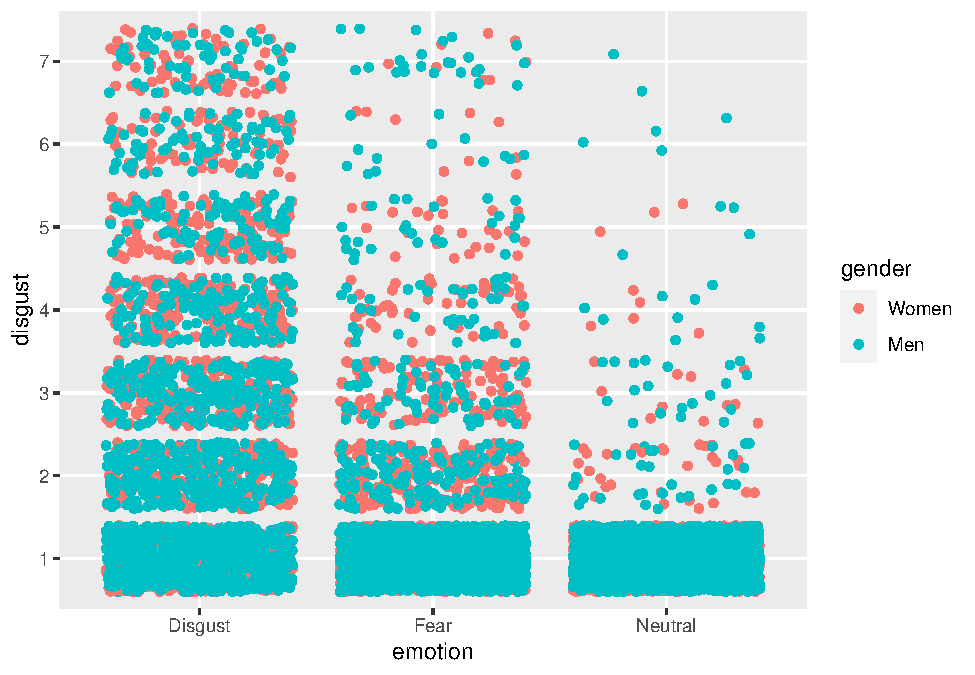
\includegraphics{DAP_v2_files/figure-latex/unnamed-chunk-2-1.pdf}

This figure shows the distribution of the subjective evaluation of
disgust across all pair of words, depending of the emotion elicited by
the words. As one can see, there still is a floor effect, but it seems
less strong for the disgust emotion, as one can expect.

\hypertarget{modelisation}{%
\section{Modelisation}\label{modelisation}}

Even if we have seen in our exploration that there seems to be a floor
effect, we must do a diagnostic of a linear model to certify the
inadaptation of this model to analyse our data.

\begin{Shaded}
\begin{Highlighting}[]
\NormalTok{sjPlot}\SpecialCharTok{::}\FunctionTok{plot\_model}\NormalTok{(m0,}\AttributeTok{type =} \StringTok{"diag"}\NormalTok{)[[}\DecValTok{3}\NormalTok{]]}
\end{Highlighting}
\end{Shaded}

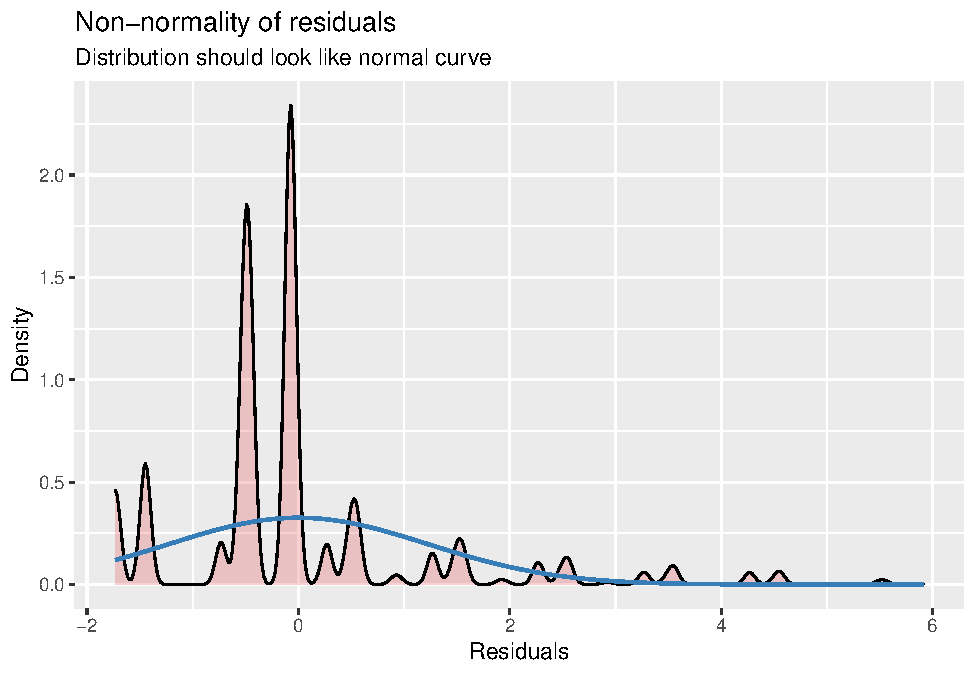
\includegraphics{DAP_v2_files/figure-latex/normal analysis of resids-1.pdf}

As expected, the residuals distribution does not follow a normal curve.
Therefore, we cannot do a classic linear regression to analyse this
data. Alternative techniques have to be investigated. (Find more
diagnostic graphs in the appendix.)

Three possible methods are being tested: (a) a simple logistic ordinal
regression, (b) a mixed-effect model considering the subjects'
repetition, and (c) a mixed-effect model considering the subjects'
repetition and the random effect of the emotions.

After modeling these methods, we can use the Akaike information
criterion to estimate the prediction error of each model, and thereby
their relative quality.

\begin{verbatim}
##         Equivalent degrees of freedom Akaike Information Criterion
## Model A                            11                     17242.03
## Model B                            12                     16204.65
## Model C                            17                     16075.78
\end{verbatim}

As shown in this table, we can conclude that the model that seems to fit
the best our data is the Model C, the mixed-effect model considering the
subjects' repetition and the random effect of the emotions, as it has
the smaller AIC, and more equivalent degrees of freedom. This being
done, we must now look for the best model using this method. According
to our initial hypothesis, we want to know if there is an impact of the
word pairs' emotion and the gender on the subjective evaluation of
disgust.

\begin{verbatim}
##                          Equivalent degrees of freedom
## Interaction Model                                   17
## Emotion and Gender Model                            15
## Model without Gender                                14
##                          Akaike Information Criterion
## Interaction Model                            16075.78
## Emotion and Gender Model                     16076.82
## Model without Gender                         16074.89
\end{verbatim}

As shown in the table above, and following the AIC estimate, the model
that fits the best to our data is the Model without Gender.

\hypertarget{model-analysis}{%
\section{Model analysis}\label{model-analysis}}

Now that we have choosen the Model without Gender as being the model
that better fits our data, we have to analyse it.

\begin{Shaded}
\begin{Highlighting}[]
\FunctionTok{summary}\NormalTok{(m3}\FloatTok{.0}\NormalTok{)}
\end{Highlighting}
\end{Shaded}

\begin{verbatim}
## Cumulative Link Mixed Model fitted with the Laplace approximation
## 
## formula: disgust ~ emotion + (emotion | subjects)
## data:    Data
## 
##  link  threshold nobs logLik   AIC      niter      max.grad cond.H 
##  logit flexible  9349 -8023.44 16074.89 1862(9330) 8.10e-03 4.9e+02
## 
## Random effects:
##  Groups   Name           Variance Std.Dev. Corr          
##  subjects (Intercept)    0.9960   0.9980                 
##           emotionFear    0.6443   0.8027   -0.050        
##           emotionNeutral 0.3974   0.6304   -0.699  0.405 
## Number of groups:  subjects 52 
## 
## Coefficients:
##                Estimate Std. Error z value Pr(>|z|)    
## emotionFear     -2.0596     0.1313  -15.68   <2e-16 ***
## emotionNeutral  -3.9909     0.1497  -26.66   <2e-16 ***
## ---
## Signif. codes:  0 '***' 0.001 '**' 0.01 '*' 0.05 '.' 0.1 ' ' 1
## 
## Threshold coefficients:
##     Estimate Std. Error z value
## 1|2  -0.5346     0.1437  -3.721
## 2|3   0.3387     0.1435   2.359
## 3|4   1.1585     0.1445   8.018
## 4|5   1.8831     0.1467  12.834
## 5|6   2.6467     0.1515  17.466
## 6|7   3.4641     0.1619  21.402
\end{verbatim}

\begin{Shaded}
\begin{Highlighting}[]
\NormalTok{(ctable }\OtherTok{\textless{}{-}} \FunctionTok{coef}\NormalTok{(}\FunctionTok{summary}\NormalTok{(m3}\FloatTok{.0}\NormalTok{)))}
\end{Highlighting}
\end{Shaded}

\begin{verbatim}
##                  Estimate Std. Error    z value      Pr(>|z|)
## 1|2            -0.5345518  0.1436559  -3.721058  1.983896e-04
## 2|3             0.3386870  0.1435477   2.359404  1.830430e-02
## 3|4             1.1585096  0.1444951   8.017640  1.077963e-15
## 4|5             1.8831354  0.1467277  12.834219  1.054604e-37
## 5|6             2.6466679  0.1515367  17.465527  2.622672e-68
## 6|7             3.4641486  0.1618577  21.402428 1.268284e-101
## emotionFear    -2.0595720  0.1313485 -15.680213  2.065598e-55
## emotionNeutral -3.9909173  0.1496919 -26.660871 1.338921e-156
\end{verbatim}

That means that the word pairs' emotion explains the disgust evaluation
(p\textless{} 0.001).

The estimated model can be written as:
\[Logit(P(Y\le 2))= (-0.5346) - (-2.0596)*emotionFear - (-3.9909)*emotionNeutral\]
\[Logit(P(Y\le 3))= 0.3387 - (-2.0596)*emotionFear - (-3.9909)*emotionNeutral\]
\[Logit(P(Y\le 4))= 1.1585 - (-2.0596)*emotionFear - (-3.9909)*emotionNeutral\]
\[Logit(P(Y\le 5))= 1.8831 - (-2.0596)*emotionFear - (-3.9909)*emotionNeutral\]
\[Logit(P(Y\le 6))= 2.6467 - (-2.0596)*emotionFear - (-3.9909)*emotionNeutral\]
\[Logit(P(Y\le 7))= 3.4641 - (-2.0596)*emotionFear - (-3.9909)*emotionNeutral\]

Being the model that best fits the data doesn't mean that it's a good
model, that is why we must check for the effect size.

~

disgust

Predictors

Odds Ratios

CI

p

1\textbar2

0.59

0.44~--~0.78

\textless0.001

2\textbar3

1.40

1.06~--~1.86

0.018

3\textbar4

3.19

2.40~--~4.23

\textless0.001

4\textbar5

6.57

4.93~--~8.76

\textless0.001

5\textbar6

14.11

10.48~--~18.99

\textless0.001

6\textbar7

31.95

23.26~--~43.88

\textless0.001

emotion {[}Fear{]}

0.13

0.10~--~0.16

\textless0.001

emotion {[}Neutral{]}

0.02

0.01~--~0.02

\textless0.001

Random Effects

σ2

3.29

τ00 subjects

1.00

τ11 subjects.emotionFear

0.64

τ11 subjects.emotionNeutral

0.40

ρ01

-0.05

-0.70

ICC

0.24

N subjects

52

Observations

9349

Marginal R2 / Conditional R2

0.381 / 0.528

In this table, we can see that the Conditional R\^{}2 is 0.528, which
means that the model explains 52,8\% of the variance explained by both
the fixed and random factors.

\hypertarget{diagnostic-of-the-model}{%
\section{Diagnostic of the model}\label{diagnostic-of-the-model}}

\begin{Shaded}
\begin{Highlighting}[]
\CommentTok{\#read this : David W.. Hosmer, Lemeshow, S., \& Rodney X.. Sturdivant. (2000). Applied logistic regression. New York: Wiley. {-}{-}\textgreater{} §5}

\FunctionTok{autoplot.clm}\NormalTok{(m1}\FloatTok{.2}\NormalTok{)}
\end{Highlighting}
\end{Shaded}

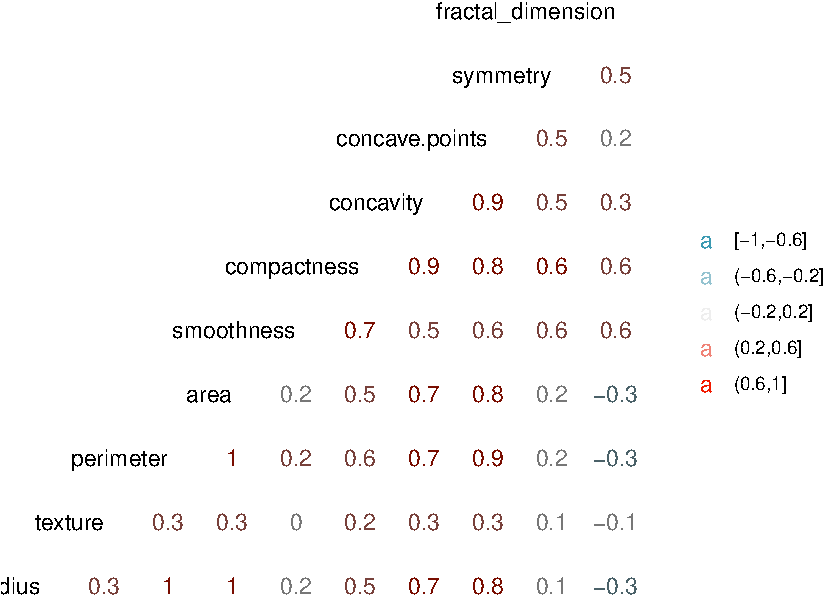
\includegraphics{DAP_v2_files/figure-latex/unnamed-chunk-7-1.pdf}

\begin{Shaded}
\begin{Highlighting}[]
\FunctionTok{plot}\NormalTok{(m0, }\AttributeTok{which =} \DecValTok{2}\NormalTok{)}
\end{Highlighting}
\end{Shaded}

\includegraphics{DAP_v2_files/figure-latex/unnamed-chunk-7-2.pdf}

\hypertarget{conclusion}{%
\section{Conclusion}\label{conclusion}}

The present data analysis was aimed to analyse and compare three
statistical methods to analyse a dataset that

\end{document}
